% Compilation : pdflatex Dynamique_des_fluides_visqueux_v4.tex (deux fois).
% Document autonome : texte, formules et figures TikZ modifiables.
% Les reperes Source renvoient aux pages du manuscrit.
\documentclass[11pt,a4paper]{article}
\usepackage[utf8]{inputenc}
\usepackage[T1]{fontenc}
\usepackage[provide=*,french]{babel}
\usepackage[scaled=.95]{helvet}
\renewcommand{\familydefault}{\sfdefault}
\usepackage{amsmath,amssymb,esint,array,tabularx}
\usepackage{geometry}
\geometry{left=15mm,right=15mm,top=18mm,bottom=18mm,headheight=14pt,headsep=6mm}
\usepackage{fancyhdr,lastpage,tikz}
\usetikzlibrary{arrows.meta,calc,decorations.pathreplacing,decorations.pathmorphing,decorations.markings,patterns}
\usepackage[most]{tcolorbox}
\usepackage{enumitem,titlesec,needspace,hyperref}
\hypersetup{hidelinks,pdftitle={Dynamique des fluides visqueux},pdfsubject={Cours de physique}}
\pagestyle{fancy}\fancyhf{}
\fancyhead[L]{\small Physique F3 - Dynamique des fluides visqueux - inspiré par les cours de Mme Mesnil}
\fancyhead[R]{\small\thepage/\pageref{LastPage}}
\fancyfoot[R]{\small PC-PC*}
\renewcommand{\headrulewidth}{0pt}
\clubpenalty=10000\widowpenalty=10000\displaywidowpenalty=10000
\setlength{\parindent}{0pt}\setlength{\parskip}{4pt}
\setlength{\abovedisplayskip}{6pt}\setlength{\belowdisplayskip}{6pt}
\AtBeginEnvironment{center}{\setlength{\topsep}{4pt}\setlength{\partopsep}{0pt}}
\setlist[itemize]{leftmargin=5mm,itemsep=3pt,topsep=3pt,label=\(\rightarrow\)}
\setlist[enumerate]{leftmargin=6mm,itemsep=3pt,topsep=3pt}
\renewcommand{\thesection}{\Roman{section}}
\renewcommand{\thesubsection}{\thesection.\arabic{subsection}}
\titleformat{\section}{\Large\bfseries}{\thesection.}{.4em}{}
\titleformat{\subsection}{\large\bfseries}{\thesubsection.}{.4em}{}[\titlerule]
\titleformat{\subsubsection}{\normalsize\bfseries}{\alph{subsubsection})}{.5em}{}
\titlespacing*{\section}{0pt}{11pt}{6pt}
\titlespacing*{\subsection}{0pt}{9pt}{5pt}
\titlespacing*{\subsubsection}{0pt}{8pt}{4pt}
\newtcolorbox{cadre}[1][]{enhanced,sharp corners,colback=white,colframe=black,boxrule=1.1pt,left=7pt,right=7pt,top=5pt,bottom=5pt,before skip=7pt,after skip=7pt,#1}
\newtcolorbox{exemple}[1][]{enhanced,sharp corners,colback=white,colframe=black,boxrule=.7pt,left=8pt,right=8pt,top=6pt,bottom=6pt,before skip=8pt,after skip=8pt,#1}
\tcbset{etoiles/.style={width=\dimexpr\linewidth-22mm\relax,overlay={\node[anchor=west,inner sep=0pt,font=\small] at ([xshift=2mm]frame.east) {\(#1\)};}}}
\newcommand{\dd}{\mathrm d}
\newcommand{\vv}{\vec v}
\newcommand{\grad}{\overrightarrow{\mathrm{grad}}}
\newcommand{\pd}[2]{\frac{\partial #1}{\partial #2}}
\newcommand{\ux}{\vec u_x}\newcommand{\uy}{\vec u_y}\newcommand{\uz}{\vec u_z}
\newcommand{\cste}{\mathrm{cste}}
\newcommand{\titr}[1]{\par\textbf{\underline{#1}}\par\nopagebreak[3]}
\newcommand{\planpart}[2]{\par\vspace{5pt}{\bfseries #1. #2}\par}
\newcommand{\plansub}[2]{\hspace*{7mm}{\itshape #1) #2}\par}
\newcommand{\plansubsub}[1]{\hspace*{15mm}{\itshape #1}\par}
\tikzset{>=Stealth,every node/.style={font=\small},flow/.style={thick,->},edge/.style={thick}}
\newcommand{\etoiles}[1]{\foreach \i in {1,...,#1}{\mathord{\star}\,}}
\newcommand{\R}{\mathcal R}
\newcommand{\Dv}{\frac{\mathrm D\vec v}{\mathrm Dt}}
\newcommand{\conv}{(\vec v\cdot\grad)\vec v}
\newcommand{\fv}{\vec f_v}\newcommand{\fvt}{\vec f_{v,\mathrm{tot}}}\newcommand{\fvi}{\vec f_{v,\mathrm{inertie}}}
\newcommand{\diver}{\operatorname{div}}
\newcommand{\Rey}{R_e}
\newcommand{\cv}{\underline{v_x}}\newcommand{\cf}{\underline f}
\newcommand{\rep}{\draw[->] (0,0)--(1,0);\draw[->] (0,0)--(0,1);\draw[->] (0,0)--(-.5,-.6);\node[below right] at (.25,-.15){$\R$};}
\newcommand{\circuit}{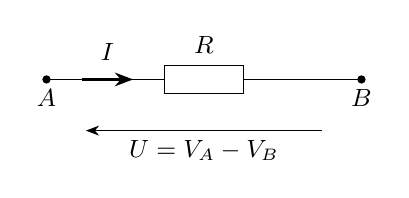
\begin{tikzpicture}
\fill (0,0) circle(1.5pt) node[below]{$A$};\fill (4,0) circle(1.5pt) node[below]{$B$};\draw (0,0)--(1.5,0) (2.5,0)--(4,0);\draw (1.5,-.18) rectangle(2.5,.18);\node[above] at (2,.2){$R$};\draw[->,thick] (.45,0)--(1.1,0) node[midway,above=3pt]{$I$};\draw[->] (3.5,-.65)--(.5,-.65) node[midway,below]{$U=V_A-V_B$};
\end{tikzpicture}}
% Profils de vitesse : 0 Couette ; 1 Poiseuille plan ; 2 Poiseuille cylindrique.
\newcommand{\profil}[1]{\begin{tikzpicture}[scale=.85]
\ifnum#1<2
\draw[->] (0,0)--(5.5,0) node[right]{$x$};\draw[->] (0,0)--(0,3) node[above]{$z$};\draw[thick] (0,2.4)--(5.1,2.4);\node[left] at (0,2.4){$e$};
\ifnum#1=0
\draw[thick] (0,0)--(3.8,2.4);\foreach \z in {.3,.6,.9,1.2,1.5,1.8,2.1}{\draw[->] (0,\z)--({3.8*\z/2.4},\z);}\node[above right] at (3.8,2.4){$\vec v_0$};
\else
\draw[thick,domain=0:2.4,samples=50,variable=\z] plot({1.7*\z*(2.4-\z)},\z);
\foreach \z in {.2,.5,.8,1.1,1.4,1.7,2,2.2}{\draw[->] (0,\z)--({1.7*\z*(2.4-\z)},\z);}
\draw[dashed] (0,1.2)--(2.65,1.2);\node[left] at (0,1.2){$e/2$};\node at (4,1.2){Profil parabolique};\node[below left] at (0,0){$O$};
\fi
\else
\draw[->] (0,0)--(5.5,0) node[right]{$z$};\draw (0,-1.6)--(0,1.6);\draw[thick] (0,-1.2)--(5,-1.2) (0,1.2)--(5,1.2);
\draw[thick,domain=-1.2:1.2,samples=50,variable=\r] plot({1.7*(1.44-\r*\r)},\r);
\foreach \r in {-1,-.75,-.5,-.25,.25,.5,.75,1}{\draw[->] (0,\r)--({1.7*(1.44-\r*\r)},\r);}\node at (3.9,-.65){Profil parabolique};
\fi\end{tikzpicture}}
% Tube et, selon le cas, lignes de courant (1) ou section de debit (2).
\newcommand{\tube}[1]{\begin{tikzpicture}[scale=.9]
\draw[thick] (0,-.9)--(4.7,-.9) (0,.9)--(4.7,.9);\draw (0,0) ellipse(.33 and .9);
\draw (4.7,.9) arc(90:270:.33 and .9);\draw[dashed] (4.7,-.9) arc(-90:90:.33 and .9);
\draw[dashed,->] (-1,0)--(5.8,0) node[right]{$Oz$};\fill (0,0) circle(1.5pt) node[below left=3pt,fill=white,inner sep=1pt]{$A$};\fill (4.7,0) circle(1.5pt) node[below right=5pt,fill=white,inner sep=1pt]{$B$};
\draw[<->] (0,-1.3)--(4.7,-1.3) node[midway,below]{$L$};\draw[<->] (5.35,0)--(5.35,.9) node[midway,right]{$R$};
\draw[->,thick] (.6,.45)--(1.5,.45);
\ifnum#1=1\foreach \y in {-.6,-.3,.3,.6}{\draw[->] (.25,\y)--(4.4,\y);}\fi
\ifnum#1=2\fill[pattern=north east lines,pattern color=gray] (2.5,0) ellipse(.33 and .9);\draw (2.5,0) ellipse(.33 and .9);\draw[thick] (2.5,0) ellipse(.16 and .42);\fi
\end{tikzpicture}}
% Volume cylindrique pour les deux exemples : anneau (1), cylindre plein (2).
\newcommand{\volumeex}[1]{\begin{tikzpicture}[scale=.85]
\draw[->] (-1.5,0)--(3.2,0) node[right]{$z$};
\ifnum#1=1
\fill[blue!12] (0,-1)--(.6,-1) arc(-90:90:.38 and 1)--(0,1) arc(90:270:.38 and 1);
\fill[blue!25,even odd rule] (0,0) ellipse(.38 and 1) (0,0) ellipse(.26 and .7);
\fill[blue!25,even odd rule] (.6,0) ellipse(.38 and 1) (.6,0) ellipse(.26 and .7);
\filldraw[fill=white] (0,0) ellipse(.26 and .7);\filldraw[fill=white] (.6,0) ellipse(.26 and .7);
\draw (0,.7)--(.6,.7) (0,-.7)--(.6,-.7);
\draw[thin] (.85,.7)--(1.7,.7) (.95,1)--(1.7,1);
\draw[<->] (1.55,.7)--(1.55,1) node[right=3pt,midway]{$\dd r$};
\else
\fill[blue!12] (0,-1)--(.6,-1) arc(-90:90:.38 and 1)--(0,1) arc(90:270:.38 and 1);
\fill[blue!25] (0,0) ellipse(.38 and 1);
\fi
\draw[thick] (0,0) ellipse(.38 and 1);\draw[thick] (.6,0) ellipse(.38 and 1);\draw (0,1)--(.6,1) (0,-1)--(.6,-1);
\draw[thin] (0,-1.15)--(0,-1.65) (.6,-1.15)--(.6,-1.65);
\draw[<->] (0,-1.55)--(.6,-1.55) node[midway,below]{$\dd z$};
\ifnum#1=1\def\rad{.7}\else\def\rad{1}\fi
\draw[<->] (2.25,0)--(2.25,\rad) node[midway,right]{$r$};
\foreach \y in {-.5,.5}{\draw[-{Stealth[length=3pt]}] (-.75,\y)--(-.36,\y);\draw[-{Stealth[length=3pt]}] (1.3,\y)--(.96,\y);}
\draw[-{Stealth[length=3pt]}] (.3,1.32)--(.3,1.02);
\draw[-{Stealth[length=3pt]}] (.3,-1.32)--(.3,-1.02);
\end{tikzpicture}}
\begin{document}
{\raggedright\fontsize{27}{31}\selectfont\bfseries Dynamique des fluides visqueux\par}
\vspace{4mm}
\begingroup\setlength{\parskip}{.7pt}
\planpart{I}{Équation de Navier--Stokes}
\plansub{1}{Équation de Navier--Stokes}
\plansub{2}{Transport de quantité de mouvement}
\plansub{3}{Nombre de Reynolds}
\planpart{II}{Écoulement de Couette plan}
\planpart{III}{Écoulement de Poiseuille}
\plansub{1}{Écoulement de Poiseuille plan}
\plansub{2}{Écoulement de Poiseuille cylindrique}
\planpart{IV}{Plaque oscillante}
\endgroup

% Source 1
Dans tout ce chapitre, on suppose que l'écoulement est incompressible et que le fluide est newtonien. La force de viscosité exercée sur une particule fluide s'écrit
\begin{cadre}\[\dd^3\vec f_{\mathrm{vis}}=\eta\Delta\vec v\,\dd^3\tau.\]\end{cadre}
\section{Équation de Navier--Stokes}
\subsection{Équation de Navier--Stokes}
\begin{center}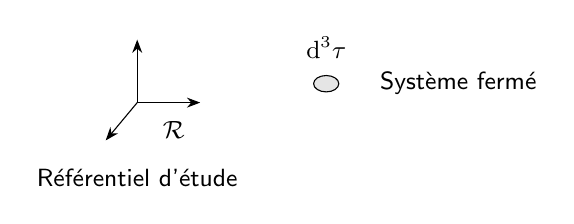
\begin{tikzpicture}[scale=.8]
\rep\node[below] at (0,-.9){Référentiel d'étude};\fill[gray!20] (3,.3) ellipse(.2 and .13);\draw (3,.3) ellipse(.2 and .13);\node[above] at (3,.55){$\dd^3\tau$};\node[right] at (3.7,.3){Système fermé};
\end{tikzpicture}\end{center}
Le théorème de la quantité de mouvement donne
\[\mu\dd^3\tau\,\Dv=\underbrace{\fv\dd^3\tau}_{\text{forces à distance}}+\underbrace{\bigl(-\grad P\,\dd^3\tau+\eta\Delta\vec v\,\dd^3\tau\bigr)}_{\text{forces de contact}}+\underbrace{\dd^3\vec f_{\mathrm{inertie}}}_{\fvi\dd^3\tau}.\]
% Source 2
\begin{cadre}[etoiles={\etoiles{5}}]
\textbf{Équation de Navier--Stokes :}
\[\mu\Dv=\underbrace{\bigl(\fv+\fvi\bigr)}_{\fvt}-\grad P+\eta\Delta\vec v.\]
\end{cadre}
\subsection{Transport de quantité de mouvement}
\[\mu\pd{\vec v}{t}+\mu\conv=\fvt-\grad P+\eta\Delta\vec v.\]
Ainsi,
\[\pd{\vec v}{t}=-\underbrace{\conv}_{\substack{\text{transport de quantité de}\\\text{mouvement par convection}}}+\underbrace{\frac\eta\mu\Delta\vec v}_{\substack{\text{transport de quantité de}\\\text{mouvement par diffusion}}}+\frac1\mu\fvt-\frac1\mu\grad P.\]
\titr{Cas où le terme $\dfrac\eta\mu\Delta\vec v$ est prépondérant}
\[\pd{\vec v}{t}=\frac\eta\mu\Delta\vec v.\]
\begin{cadre}[etoiles={\etoiles{4}}]\[\pd{\vec v}{t}=\nu\Delta\vec v.\]\textbf{Équation de la diffusion.}\end{cadre}
% Source 3
Avec $\nu=\eta/\mu$, coefficient de viscosité cinématique, qui est un coefficient de diffusion. Unité : $\mathrm{m^2\,s^{-1}}$.
\begin{center}\renewcommand{\arraystretch}{1.55}\begin{tabular}{c|c|c|c}
& Glycérine & Eau & Air\\\hline
$\mu$ & $1\times10^3\,\mathrm{kg\,m^{-3}}$ & $1\times10^3\,\mathrm{kg\,m^{-3}}$ & $1\,\mathrm{kg\,m^{-3}}$\\
$\eta$ & $1\,\mathrm{Pl}$ & $1\times10^{-3}\,\mathrm{Pl}$ & $1\times10^{-5}\,\mathrm{Pl}$\\
$\nu$ & $1\times10^{-3}\,\mathrm{m^2\,s^{-1}}$ & $1\times10^{-6}\,\mathrm{m^2\,s^{-1}}$ & $1\times10^{-5}\,\mathrm{m^2\,s^{-1}}$
\end{tabular}\end{center}
$\nu_{\mathrm{air}}>\nu_{\mathrm{eau}}$ : l'eau est plus visqueuse que l'air, mais le transport de quantité de mouvement est plus efficace dans l'air. Deux phénomènes interviennent : la viscosité et l'inertie.

\subsection{Nombre de Reynolds}
On compare le transport de quantité de mouvement par convection et par diffusion.
% Source 4
\begin{cadre}\[\Rey=\frac{\mu\bigl\|\conv\bigr\|}{\bigl\|\eta\Delta\vec v\bigr\|}.\]\end{cadre}
\titr{Grandeurs caractéristiques de l'écoulement}
\begin{center}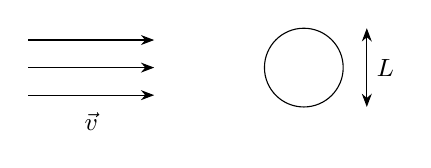
\begin{tikzpicture}
\foreach \y in {-.35,0,.35}{\draw[->] (0,\y)--(1.6,\y);}\node[below] at (.8,-.45){$\vec v$};\draw (3.5,0) circle(.5);\draw[<->] (4.3,-.5)--(4.3,.5) node[midway,right]{$L$};
\end{tikzpicture}\end{center}
Les grandeurs caractéristiques sont la vitesse $v$, la masse volumique $\mu$, la viscosité $\eta$ et la taille caractéristique $L$.

\textbf{Hypothèse :} il existe une seule distance caractéristique $L$.
\[\mu\left[\pd{\vec v}{t}+\underbrace{\conv}_{\text{non linéaire}}\right]=\fvt-\grad P+\eta\Delta\vec v.\]
% Source 5
Cette équation non linéaire est difficile à résoudre. Un enjeu en mécanique des fluides est de simplifier l'équation de Navier--Stokes à partir des ordres de grandeur.
\begin{center}\begin{tikzpicture}[scale=.8]
\draw[->] (0,0)--(4,0) node[right]{$x$};\draw[->] (0,0)--(0,2.4) node[above]{$f(x)$};\draw[thick] (.7,.6)..controls (1.4,1.5) and (2.2,1.9)..(3.1,2.1);\draw[<->] (.7,.35)--(3.1,.35) node[midway,above]{$L$};
\end{tikzpicture}\end{center}
En ordre de grandeur, $f'(x)\simeq f/L$. Ainsi,
\[\conv\simeq v\frac vL,\qquad\Delta\vec v\simeq\frac v{L^2}.\]
\begin{cadre}[etoiles={\etoiles{5}}]\[\Rey=\frac{\mu v\dfrac vL}{\eta\dfrac v{L^2}}=\frac{\mu vL}{\eta}.\]\end{cadre}
\begin{itemize}
\item Si $\Rey\gg1$, le transport de quantité de mouvement par convection est très supérieur au transport par diffusion.
\item Si $\Rey\ll1$, le transport de quantité de mouvement par convection est très inférieur au transport par diffusion.
\end{itemize}
% Source 6
\textbf{Remarque :} Un souffle sur un disque de rayon $R$ fait intervenir deux tailles caractéristiques.
\begin{center}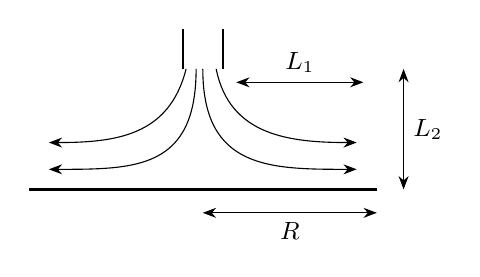
\begin{tikzpicture}[scale=.85]
\draw[thick] (-.3,2.4)--(-.3,1.8) (.3,2.4)--(.3,1.8);\draw[thick] (-2.6,0)--(2.6,0);\draw[->] (0,1.8)..controls (0,.3) and (1,.3)..(2.3,.3);\draw[->] (.2,1.8)..controls (.4,.8) and (1.3,.7)..(2.3,.7);\draw[->] (-.1,1.8)..controls (-.1,.3) and (-1,.3)..(-2.3,.3);\draw[->] (-.25,1.8)..controls (-.5,.8) and (-1.3,.7)..(-2.3,.7);\draw[<->] (.5,1.6)--(2.4,1.6) node[midway,above]{$L_1$};\draw[<->] (3,0)--(3,1.8) node[midway,right]{$L_2$};\draw[<->] (0,-.35)--(2.6,-.35) node[midway,below]{$R$};
\end{tikzpicture}\end{center}
Le nombre de Reynolds généralisé sera étudié au cas par cas dans les exercices. Cf. exercice 1 du TD.
\[\mu\Dv=\fvt-\grad P+\eta\Delta\vec v.\]
Si le fluide est au repos, $\vec v=\vec0$ : il n'y a pas de force de viscosité.
\begin{cadre}\[\vec0=\fvt-\grad P.\]\textbf{Statique des fluides.}\end{cadre}
% Sources 6-10
\section{Écoulement de Couette plan}
\Needspace{100pt}\titr{Dispositif}
\begin{center}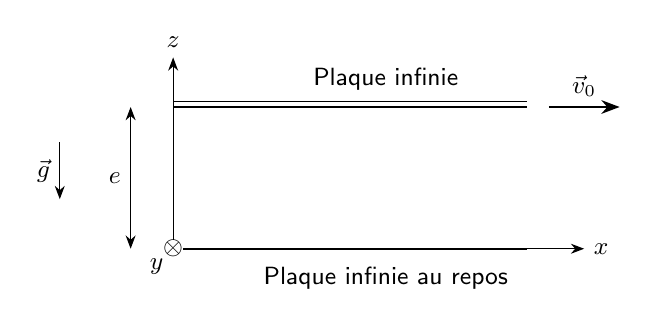
\begin{tikzpicture}[scale=.9]
\draw[thick] (0,0)--(5,0);\draw[thick] (0,2)--(5,2);\draw (0,2.08)--(5,2.08);\draw[->] (0,0)--(5.8,0) node[right]{$x$};\draw[->] (0,0)--(0,2.7) node[above]{$z$};\node[fill=white,inner sep=0pt] at (0,0){$\otimes$};\node[below left] at (0,0){$y$};
\draw[<->] (-.6,0)--(-.6,2) node[midway,left]{$e$};\draw[->,thick] (5.3,2)--(6.3,2) node[midway,above]{$\vec v_0$};\node[above] at (3,2.1){Plaque infinie};\node[below] at (3,-.12){Plaque infinie au repos};\draw[->] (-1.6,1.5)--(-1.6,.7) node[midway,left]{$\vec g$};
\end{tikzpicture}\end{center}
L'écoulement est généré par le mouvement de la plaque supérieure, de vitesse $v_0\ux$. Il n'y a pas de gradient de pression parallèle à $(Ox)$ : $\partial P/\partial x=0$.

L'objectif est de déterminer $P(M)$ et $\vec v(M,t)$.
\titr{Hypothèses}
\begin{itemize}
\item L'écoulement est stationnaire : $\vec v(M)$ et $P(M)$ ne dépendent pas du temps. Le temps d'observation est supérieur à la durée du régime transitoire.
\item L'écoulement est laminaire : $\vec v=v_x\ux$.
\end{itemize}
\titr{Calcul de $\vec v$}
\[P(M)=P(x,y,z),\qquad\vec v(M)=v_x(x,y,z)\ux.\]
Les plaques sont considérées comme infinies : $e$ est très petit devant leur taille. Le dispositif est invariant par translation parallèlement à $(Ox)$ et à $(Oy)$.
\begin{cadre}\[P(M)=P(z),\qquad\vec v(M)=v_x(z)\ux.\]\end{cadre}
\textbf{Remarque :} $\diver\vec v=\partial v_x/\partial x=0$ : l'écoulement est bien incompressible.

Le référentiel d'étude est celui du laboratoire, supposé galiléen. L'équation de Navier--Stokes s'écrit
\begin{cadre}\[\mu\Dv=\mu\vec g-\grad P+\eta\Delta\vec v.\]\end{cadre}
\begin{align*}
\Dv&=\pd{\vec v}{t}+\conv\\
&=\vec0+\left(v_x\frac\partial{\partial x}+\underbrace{v_y}_{0}\frac\partial{\partial y}+\underbrace{v_z}_{0}\frac\partial{\partial z}\right)(v_x\ux).
\end{align*}
\begin{cadre}\[\Dv=v_x\frac\partial{\partial x}\bigl[v_x(z)\ux\bigr]=\vec0.\]\end{cadre}
La particule de fluide est pseudo-isolée.

\titr{Projection de l'équation de Navier--Stokes}
\[\Delta\vec v=\begin{pmatrix}\displaystyle\Delta v_x=\underbrace{\frac{\partial^2v_x}{\partial x^2}}_{0}+\underbrace{\frac{\partial^2v_x}{\partial y^2}}_{0}+\frac{\partial^2v_x}{\partial z^2}\\[14pt]\Delta v_y=0\\[6pt]\Delta v_z=0\end{pmatrix}.\]
\[\begin{aligned}
\ux:\quad0&=-\underbrace{\pd P x}_{0}+\eta\frac{\partial^2v_x}{\partial z^2},&&\text{(1)}\\[7pt]
\uy:\quad0&=-\underbrace{\pd P y}_{0},\\[7pt]
\uz:\quad0&=-\mu g-\pd P z.&&\text{(3)}
\end{aligned}\]
L'équation (3) donne
\begin{cadre}\[P(z)=-\mu gz+\cste.\]\end{cadre}
L'équation (1) donne $\partial^2v_x/\partial z^2=0$, d'où
\begin{cadre}\[v_x(z)=Az+B.\]\end{cadre}
\titr{Conditions limites cinématiques}
\[v_x(0)=0,\qquad v_x(e)=v_0\qquad\Longrightarrow\qquad B=0,\quad A=\frac{v_0}e.\]
\titr{Conclusion}
\begin{cadre}\[\vec v(M)=\frac{v_0z}e\ux.\]\end{cadre}
\begin{center}\profil{0}\end{center}
\textbf{Remarque :} A posteriori, une application numérique permet de vérifier que $\Rey<1$.

% Sources 10-15
\section{Écoulement de Poiseuille}
\subsection{Écoulement de Poiseuille plan}
\begin{center}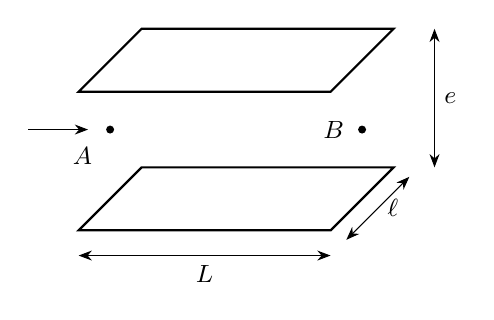
\begin{tikzpicture}[scale=.8]
\draw[thick] (0,0)--(4,0)--(5,1)--(1,1)--cycle;\draw[thick] (0,2.2)--(4,2.2)--(5,3.2)--(1,3.2)--cycle;
\fill (.5,1.6) circle(1.8pt) node[below left=3pt]{$A$};\fill (4.5,1.6) circle(1.8pt) node[left=3pt]{$B$};\draw[->] (-.8,1.6)--(.15,1.6);
\draw[<->] (0,-.4)--(4,-.4) node[midway,below]{$L$};\draw[<->] (4.25,-.15)--(5.25,.85) node[midway,right]{$\ell$};\draw[<->] (5.65,1)--(5.65,3.2) node[midway,right]{$e$};
\end{tikzpicture}\end{center}
$P_A>P_B$ : l'écoulement se fait de $A$ vers $B$.
\begin{center}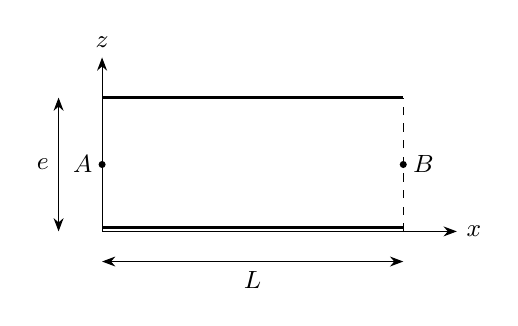
\begin{tikzpicture}[scale=.85]
\draw[->] (0,0)--(5.3,0) node[right]{$x$};\draw[->] (0,0)--(0,2.6) node[above]{$z$};\draw[thick] (0,.06)--(4.5,.06) (0,2)--(4.5,2);\draw[dashed] (4.5,0)--(4.5,2);\fill (0,1) circle(1.5pt) node[left]{$A$};\fill (4.5,1) circle(1.5pt) node[right]{$B$};\draw[<->] (-.65,0)--(-.65,2) node[midway,left]{$e$};\draw[<->] (0,-.45)--(4.5,-.45) node[midway,below]{$L$};
\end{tikzpicture}\end{center}
\titr{Hypothèses}
\begin{itemize}
\item $\ell\gg e$ et $\ell\gg L$ : le dispositif est invariant par translation parallèlement à $(Oy)$. Ainsi, $P(M,t)=P(x,z,t)$ et $\vec v(M,t)=\vec v(x,z,t)$.
\item Le régime est permanent : $P$ et $\vec v$ ne dépendent pas du temps.
\item L'écoulement est laminaire : $\vec v(M)=v_x(x,z)\ux$.
\item La pesanteur est négligée : $\mu g\ll\|\grad P\|$ et $\mu g\ll\|\eta\Delta\vec v\|$.
\end{itemize}
Donc $P(M)=P(x,z)$ et $\vec v(M)=v_x(x,z)\ux$.
L'incompressibilité de l'écoulement impose $\diver\vec v=0=\partial v_x/\partial x$.
\begin{cadre}\[\vec v(M)=v_x(z)\ux.\]\end{cadre}
Ainsi, $\partial^2v_x/\partial z^2=\dd^2v_x/\dd z^2$.

\Needspace{65pt}\titr{Conditions limites}
\begin{itemize}
\item Conditions limites dynamiques : $P(A)=P_A$ et $P(B)=P_B$.
\item Conditions limites cinématiques : $v_x(0)=v_x(e)=0$.
\end{itemize}

\titr{Équation de Navier--Stokes}
\[\mu\left[\pd{\vec v}{t}+\conv\right]=-\grad P+\eta\Delta\vec v.\]
Sa projection donne
\[\begin{aligned}
x:\quad0&=-\pd P x+\eta\frac{\partial^2v_x}{\partial z^2},\\[5pt]
y:\quad0&=0+0,\\[5pt]
z:\quad0&=-\pd P z\quad\Longrightarrow\quad P(M)=P(x),\quad\pd P x=\frac{\dd P}{\dd x}.
\end{aligned}\]
Donc, pour tous $x$ et $z$,
\[\underbrace{\frac{\dd P}{\dd x}}_{\text{fonction de }x}=\underbrace{\eta\frac{\dd^2v_x}{\dd z^2}}_{\text{fonction de }z}.\]
Les deux membres sont donc égaux à une constante $k$ :
\[\frac{\dd P}{\dd x}=\eta\frac{\dd^2v_x}{\dd z^2}=k,\qquad P(x)=kx+A.\]
Avec les conditions limites dynamiques,
\begin{cadre}\[P(x)=P_A+\frac{P_B-P_A}Lx,\qquad k=\frac{P_B-P_A}L.\]\end{cadre}
\[\frac{\dd^2v_x}{\dd z^2}=\frac k\eta=\frac{P_B-P_A}{\eta L},\qquad v_x(z)=\frac{P_B-P_A}{2\eta L}z^2+Bz+C.\]
Avec les conditions limites cinématiques,
\begin{cadre}\[v_x(z)=\frac{P_B-P_A}{2\eta L}z(z-e).\]\end{cadre}
\begin{center}\profil{1}\end{center}
$P_A>P_B$, donc $P_B-P_A<0$ : le coefficient de la parabole est négatif.

\titr{Débit volumique}
\[D_V=\iint_{\text{dispositif}}\vec v\cdot\dd^2\vec S=\ell\int_0^e v_x(z)\,\dd z,\]
avec $z$ variant de $0$ à $e$, et la coordonnée dans la largeur de $0$ à $\ell$.
\begin{align*}
D_V&=\ell\frac{P_B-P_A}{2\eta L}\int_0^e(z^2-ze)\,\dd z\\
&=\frac{P_B-P_A}{2\eta L}\ell\left(\frac{e^3}3-\frac{e^3}2\right).
\end{align*}
\begin{cadre}\[D_V=\frac{P_A-P_B}{12\eta L}\ell e^3>0.\]\end{cadre}
Le débit est proportionnel à $e^3$. Il diminue lorsque $\eta$ augmente ou lorsque $L$ augmente.

\Needspace{90pt}\titr{Analogie avec la loi d'Ohm}
\begin{center}\circuit\end{center}
\[U=RI,\qquad U\longleftrightarrow P_A-P_B,\qquad I\longleftrightarrow D_V,\qquad R\longleftrightarrow R_{\mathrm{hydraulique}}.\]
\begin{cadre}\[R_{\mathrm{hydraulique}}=\frac{12\eta L}{\ell e^3}.\]\end{cadre}
La résistance hydraulique augmente si $\eta$ ou $L$ augmente, ou si $\ell$ ou $e$ diminue.

\textbf{Remarque :} Il faut vérifier a posteriori la laminarité de l'écoulement ($\Rey<1$).

% Sources 15-22
\subsection{Écoulement de Poiseuille cylindrique}
\Needspace{100pt}\titr{Dispositif}
\begin{center}\tube{0}\end{center}
La différence de pression $P_A>P_B$ génère l'écoulement.
\titr{Hypothèses}
\begin{itemize}
\item Le régime est permanent : $P(M)$ et $\vec v(M)$ ne dépendent pas du temps.
\item L'écoulement est laminaire : $\vec v(M)=v_z(r,\theta,z)\uz$.
\item La pesanteur est négligée : $\mu g\ll\|\grad P\|$ et $\mu g\ll\|\eta\Delta\vec v\|$.
\end{itemize}
\titr{Calcul de $\vec v$}
\[P(M)=P(r,\theta,z),\qquad\vec v(M)=v_z(r,\theta,z)\uz.\]
L'invariance par rotation autour de $(Oz)$ donne
\[P(M)=P(r,z),\qquad\vec v(M)=v_z(r,z)\uz.\]
L'écoulement est incompressible :
\[\diver\vec v=\underbrace{\frac1r\pd{}{r}(rv_r)}_{0}+\underbrace{\frac1r\pd{v_\theta}{\theta}}_{0}+\pd{v_z}z=0.\]
Ainsi, $\partial v_z/\partial z=0$ et
\begin{cadre}\[\vec v(M)=v_z(r)\uz.\]\end{cadre}
La pression s'écrit toujours $P(M)=P(r,z)$.

L'équation de Navier--Stokes donne
\[\mu\left[\pd{\vec v}{t}+\conv\right]=-\grad P+\eta\Delta\vec v.\]
\[\conv=\left[\underbrace{v_r}_{0}\frac\partial{\partial r}+\underbrace{v_\theta}_{0}\frac1r\frac\partial{\partial\theta}+v_z\frac\partial{\partial z}\right]\bigl[v_z(r)\uz\bigr]=\vec0.\]
\begin{cadre}\[\Dv=\vec0.\]\end{cadre}
La particule de fluide est pseudo-isolée. Les lignes de courant coïncident avec les trajectoires : chaque particule a un mouvement rectiligne uniforme.
\begin{center}\tube{1}\end{center}
\[\vec0=-\grad P+\eta\Delta\vec v,\qquad\Delta\vec v=\frac1r\frac\dd{\dd r}\left(r\frac{\dd v_z}{\dd r}\right)\uz.\]
\[\begin{aligned}
r:\quad0&=-\pd P r\quad\Longrightarrow\quad P=P(z),\\[5pt]
\theta:\quad0&=0,\\[5pt]
z:\quad0&=-\pd P z+\eta\frac1r\frac\dd{\dd r}\left(r\frac{\dd v_z}{\dd r}\right).
\end{aligned}\]
Pour tous $z$ et $r$,
\[\underbrace{\frac{\dd P}{\dd z}}_{\text{fonction de }z}=\underbrace{\eta\frac1r\frac\dd{\dd r}\left(r\frac{\dd v_z}{\dd r}\right)}_{\text{fonction de }r}.\]
Les deux membres sont égaux à une constante :
\[\frac{\dd P}{\dd z}=\frac\eta r\frac\dd{\dd r}\left(r\frac{\dd v_z}{\dd r}\right)=k.\]
Avec les conditions limites dynamiques,
\begin{cadre}\[P(z)=P_A+\frac{P_B-P_A}Lz,\qquad k=\frac{P_B-P_A}L.\]\end{cadre}
On intègre ensuite :
\begin{align*}
k&=\frac\eta r\frac\dd{\dd r}\left(r\frac{\dd v_z}{\dd r}\right),\\[4pt]
\frac{kr}\eta&=\frac\dd{\dd r}\left(r\frac{\dd v_z}{\dd r}\right),\\[4pt]
\frac{kr^2}{2\eta}+A&=r\frac{\dd v_z}{\dd r},\\[4pt]
\frac Ar+\frac{kr}{2\eta}&=\frac{\dd v_z}{\dd r},\\[4pt]
v_z(r)&=A\ln r+B+\frac{kr^2}{4\eta}.
\end{align*}
La condition limite cinématique est $v_z(R)=0$.
Lorsque $r\to0^+$, $\ln r\to-\infty$, ce qui est une absurdité physique : la vitesse ne doit pas diverger. Donc $A=0$.
\[v_z(r)=\frac k{4\eta}(r^2-R^2).\]
\begin{cadre}\[v_z(r)=\frac{P_B-P_A}{4\eta L}(r^2-R^2).\]\end{cadre}
\begin{center}\profil{2}\end{center}
\titr{Débit volumique}
\begin{center}\tube{2}\end{center}
\[D_V=\iint_{\text{section du tuyau}}\vec v\cdot\dd^2\vec S=\int_0^R v_z(r)\,2\pi r\,\dd r.\]
\begin{cadre}\[D_V=\frac{P_A-P_B}{8\eta L}\pi R^4.\]\textbf{Loi de Poiseuille.}\end{cadre}
\Needspace{90pt}\titr{Analogie avec la loi d'Ohm}
\begin{center}\circuit\end{center}
\[U\longleftrightarrow P_A-P_B,\qquad I\longleftrightarrow D_V,\qquad R\longleftrightarrow R_{\mathrm{hydraulique}},\]
\[R_{\mathrm{hydraulique}}=\frac{8\eta L}{\pi R^4}.\]
\begin{cadre}[etoiles={\etoiles{3}}]\[D_V=\frac{P_A-P_B}{R_{\mathrm{hydraulique}}}.\]\end{cadre}
\textbf{Remarques :}
\begin{itemize}
\item $D_V$ est proportionnel à $R^4$. Si $R$ est divisé par $2$, $D_V$ est divisé par $16$.
\item $R_{\mathrm{hydraulique}}$ augmente si $\eta$ ou $L$ augmente, ou si $R$ diminue.
\item L'analogie entre l'électricité et la mécanique des fluides est \textbf{purement formelle}. Les électrons dans un fil n'ont pas un profil d'écoulement parabolique.
\end{itemize}
% Sources 23-24
\titr{Remarque : expression du laplacien}
On projette l'équation de Navier--Stokes en utilisant le formulaire pour $\Delta\vec v$. On peut retrouver son expression par un bilan local, dans un écoulement de cisaillement.
\begin{center}
\makebox[214.81621pt][c]{\raisebox{0pt}[109.6769pt][0pt]{%
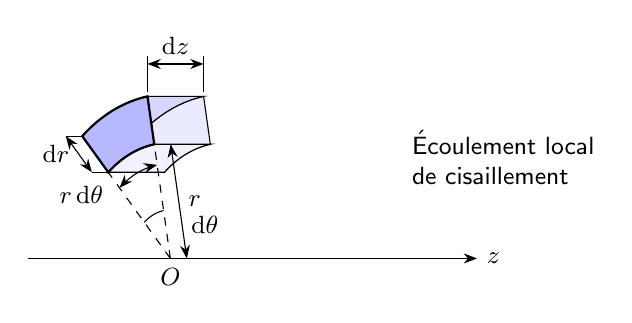
\begin{tikzpicture}[scale=.95]
% Petit secteur annulaire extrude suivant Oz.
% Projection du plan transverse : (r,theta) -> (-.8 r sin(theta),r cos(theta)).
\draw[->] (-.6,0)--(5.4,0) node[right]{$z$};
\node[below] at (1.3,0){$O$};
% Face arriere, egalement annulaire.
\filldraw[fill=blue!8] plot[domain=10:42,samples=25] ({2.05-.8*2.2*sin(\x)},{2.2*cos(\x)})
 --plot[domain=42:10,samples=25] ({2.05-.8*1.55*sin(\x)},{1.55*cos(\x)})--cycle;
% Surface cylindrique exterieure.
\filldraw[fill=blue!16] plot[domain=10:42,samples=25] ({1.3-.8*2.2*sin(\x)},{2.2*cos(\x)})
 --plot[domain=42:10,samples=25] ({2.05-.8*2.2*sin(\x)},{2.2*cos(\x)})--cycle;
% Face radiale laterale et surface cylindrique interieure.
\filldraw[fill=blue!7] ({1.3-.8*2.2*sin(42)},{2.2*cos(42)})
 --({2.05-.8*2.2*sin(42)},{2.2*cos(42)})
 --({2.05-.8*1.55*sin(42)},{1.55*cos(42)})
 --({1.3-.8*1.55*sin(42)},{1.55*cos(42)})--cycle;
\filldraw[fill=blue!5] plot[domain=10:42,samples=25] ({1.3-.8*1.55*sin(\x)},{1.55*cos(\x)})
 --plot[domain=42:10,samples=25] ({2.05-.8*1.55*sin(\x)},{1.55*cos(\x)})--cycle;
% Face avant : secteur d'anneau, avec deux arcs concentriques.
\filldraw[fill=blue!28,thick] plot[domain=10:42,samples=25] ({1.3-.8*2.2*sin(\x)},{2.2*cos(\x)})
 --plot[domain=42:10,samples=25] ({1.3-.8*1.55*sin(\x)},{1.55*cos(\x)})--cycle;
\draw[dashed] (1.3,0)--({1.3-.8*1.55*sin(10)},{1.55*cos(10)})
 (1.3,0)--({1.3-.8*1.55*sin(42)},{1.55*cos(42)});
% Rayon et epaisseur radiale, paralleles a la premiere face radiale.
\draw[<->] (1.52,0)--({1.52-.8*1.55*sin(10)},{1.55*cos(10)}) node[midway,right]{$r$};
\draw[thin] ({1.52-.8*1.55*sin(10)},{1.55*cos(10)})--({1.3-.8*1.55*sin(10)},{1.55*cos(10)})
 ({1.52-.8*2.2*sin(10)},{2.2*cos(10)})--({1.3-.8*2.2*sin(10)},{2.2*cos(10)});
\draw[thin] ({1.3-.8*1.55*sin(42)},{1.55*cos(42)})--({1.08-.8*1.55*sin(42)},{1.55*cos(42)})
 ({1.3-.8*2.2*sin(42)},{2.2*cos(42)})--({1.08-.8*2.2*sin(42)},{2.2*cos(42)});
\draw[<->] ({1.08-.8*1.55*sin(42)},{1.55*cos(42)})--({1.08-.8*2.2*sin(42)},{2.2*cos(42)}) node[midway,left]{$\dd r$};
% Angle elementaire et longueur de l'arc interieur.
\draw plot[domain=10:42,samples=20] ({1.3-.8*.65*sin(\x)},{.65*cos(\x)});
\node[right] at (1.45,.45){$\dd\theta$};
\draw[<->] plot[domain=10:42,samples=20] ({1.3-.8*1.27*sin(\x)},{1.27*cos(\x)});
\node[left] at (.53,.85){$r\,\dd\theta$};
% Epaisseur axiale.
\draw[thin] (0.994,2.23)--(0.994,2.7) (1.744,2.23)--(1.744,2.7);
\draw[<->] (0.994,2.6)--(1.744,2.6) node[midway,above]{$\dd z$};
\node[right,align=left] at (4.4,1.35){Écoulement local\\de cisaillement};
\end{tikzpicture}}}
\end{center}
\begin{align*}
\dd^3\vec f
&=\eta\left.\pd{v_z}r\right|_{r+\dd r}\dd z\,(r+\dd r)\dd\theta\,\uz-\eta\left.\pd{v_z}r\right|_r\dd z\,r\,\dd\theta\,\uz\\[5pt]
&=\eta\dd z\,\uz\,\dd\theta\left[\left.\pd{v_z}r\right|_{r+\dd r}(r+\dd r)-\left.\pd{v_z}r\right|_r r\right]\\[5pt]
&=\eta\dd z\,\uz\,\dd\theta\left[\frac\partial{\partial r}\left(r\pd{v_z}r\right)\right]\dd r\\[5pt]
&=\eta\underbrace{\dd r\,r\,\dd\theta\,\dd z}_{\dd^3\tau}\uz\left[\frac1r\frac\partial{\partial r}\left(r\pd{v_z}r\right)\right]\\[5pt]
&=\eta\dd^3\tau\underbrace{\left[\frac1r\frac\partial{\partial r}\left(r\pd{v_z}r\right)\right]\uz}_{\Delta\vec v}
=\eta\Delta\vec v\,\dd^3\tau.
\end{align*}
C.Q.F.D.

\titr{Choix d'un autre système}
Il est possible de choisir un système autre qu'une particule fluide : cette méthode est à privilégier. On choisit alors un volume de fluide différent de $\dd^3\tau$.
Puisque $\mathrm D\vec v/\mathrm Dt=\vec0$, la somme des forces est nulle :
\[\sum\vec F=\vec0,\qquad\vec f_{\mathrm{pression}}+\vec f_{\text{viscosité}}=\vec0.\]
\Needspace{140pt}\begin{exemple}[breakable]
\textbf{Premier exemple}
\begin{center}\volumeex{1}\end{center}
Le système est un anneau de fluide compris entre $r$ et $r+\dd r$, d'épaisseur $\dd z$.
\[\dd^2V=2\pi r\,\dd r\,\dd z.\]
% Source 25
Le bilan des forces s'écrit
\begin{align*}
\vec0={}&\underbrace{\eta\left.\pd{v_z}r\right|_{r+\dd r}2\pi(r+\dd r)\dd z\,\uz}_{\text{viscosité sur la surface extérieure}}
-\underbrace{\eta\left.\pd{v_z}r\right|_r2\pi r\,\dd z\,\uz}_{\text{viscosité sur la surface intérieure}}\\[6pt]
&+\underbrace{\vec0}_{\substack{\text{pression sur la}\\\text{surface extérieure}}}+\underbrace{\vec0}_{\substack{\text{pression sur la}\\\text{surface intérieure}}}
+\underbrace{P(z)\,2\pi r\,\dd r\,\uz}_{\text{pression sur la surface gauche}}
-\underbrace{P(z+\dd z)\,2\pi r\,\dd r\,\uz}_{\text{pression sur la surface droite}}.
\end{align*}
En regroupant les termes,
\begin{align*}
\vec0={}&\eta\,2\pi\,\dd z\,\uz\left[\left.\pd{v_z}r\right|_{r+\dd r}(r+\dd r)-\left.\pd{v_z}r\right|_r r\right]\\
&+2\pi r\,\dd r\,\uz\bigl[P(z)-P(z+\dd z)\bigr]\\[5pt]
={}&\eta\,2\pi\,\dd z\,\dd r\,\uz\frac\partial{\partial r}\left(r\pd{v_z}r\right)-2\pi r\,\dd r\,\uz\pd P z\,\dd z.
\end{align*}
\[\eta\frac\partial{\partial r}\left(r\pd{v_z}r\right)=r\pd P z.\]
$v_z$ ne dépend que de $r$, et $P$ ne dépend que de $z$ :
\begin{cadre}\[\eta\frac\dd{\dd r}\left(r\frac{\dd v_z}{\dd r}\right)=r\frac{\dd P}{\dd z}.\]\end{cadre}
À finir.
\end{exemple}

% Source 26
\Needspace{140pt}\begin{exemple}[breakable]
\textbf{Deuxième exemple : méthode à privilégier}
\begin{center}\volumeex{2}\end{center}
Le système est un cylindre de fluide de rayon $r$ et d'épaisseur $\dd z$, de volume
\[\dd\tau=\pi r^2\dd z.\]
Il s'agit d'un volume d'ordre 1.
Le bilan des forces donne
\begin{align*}
\vec0={}&\underbrace{\frac{\dd v_z}{\dd r}\eta\,2\pi r\,\dd z\,\uz}_{\text{viscosité de cisaillement}}+\underbrace{\vec0}_{\substack{\text{pression sur la}\\\text{surface latérale}}}\\[6pt]
&+\underbrace{P(z)\pi r^2\uz}_{\text{pression à gauche}}-\underbrace{P(z+\dd z)\pi r^2\uz}_{\text{pression à droite}}.
\end{align*}
\[\frac{\dd v_z}{\dd r}\eta\,2\pi r\,\dd z\,\uz-\frac{\dd P}{\dd z}\pi r^2\dd z\,\uz=\vec0.\]
Donc,
\begin{cadre}\[\frac{\dd P}{\dd z}\pi r^2=\eta\,2\pi r\frac{\dd v_z}{\dd r}.\]\end{cadre}
À finir.
\end{exemple}

% Sources 26-28
\section{Plaque oscillante}
On étudie un régime non stationnaire, sinusoïdal. La même méthode sera utilisée en électromagnétisme pour l'effet de peau, ainsi que pour la diffusion thermique, dans les prochains chapitres.
\Needspace{100pt}\titr{Dispositif}
\begin{center}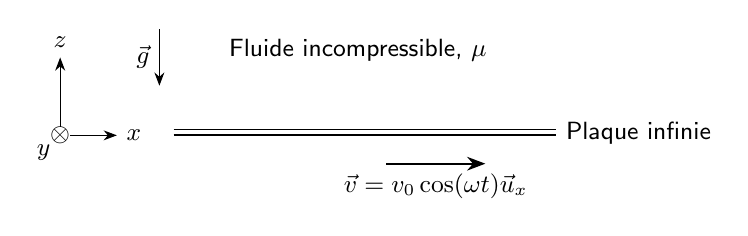
\begin{tikzpicture}[scale=.9]
\draw[->] (-1,0)--(-.2,0) node[right]{$x$};\draw[->] (-1,0)--(-1,1.1) node[above]{$z$};\node[fill=white,inner sep=0pt] at (-1,0){$\otimes$};\node[below left] at (-1,0){$y$};
\draw[thick] (.6,0)--(6,0);\draw (.6,.08)--(6,.08);\node[right] at (6,.03){Plaque infinie};\draw[->,thick] (3.6,-.4)--(5,-.4) node[midway,below]{$\vec v=v_0\cos(\omega t)\ux$};\node at (3.2,1.2){Fluide incompressible, $\mu$};\draw[->] (.4,1.5)--(.4,.7) node[midway,left]{$\vec g$};
\end{tikzpicture}\end{center}
L'objectif est de trouver $\vec v(M,t)$ pour $z>0$.
\titr{Hypothèses}
L'écoulement est laminaire. La plaque est infinie : le dispositif est invariant par translation parallèlement à $(Ox)$ et à $(Oy)$.
\[P(M,t)=P(z,t),\qquad\vec v(M,t)=v_x(z,t)\ux.\]
\textbf{Remarque :} $\diver\vec v=0$ : l'écoulement est bien incompressible.
\titr{Calcul de $\vec v$}
\[\mu\Dv=\mu\vec g-\grad P+\eta\Delta\vec v,\]
avec
\[\Dv=\pd{\vec v}{t}+\underbrace{v_x\frac\partial{\partial x}\bigl[v_x(z,t)\ux\bigr]}_{\vec0}.\]
Ainsi,
\[\mu\pd{v_x}{t}\ux=\mu\vec g-\grad P+\eta\Delta\vec v.\]
On projette :
\[\begin{aligned}
x:\quad\mu\pd{v_x}{t}&=-\underbrace{\pd P x}_{0}+\eta\frac{\partial^2v_x}{\partial z^2},\\[7pt]
y:\quad0&=0,\\[5pt]
z:\quad0&=-\pd P z-\mu g\quad\Longrightarrow\quad P=-\mu gz+\cste.
\end{aligned}\]
Donc $\mu\partial v_x/\partial t=\eta\partial^2v_x/\partial z^2$.
\begin{cadre}\[\pd{v_x}{t}=\nu\frac{\partial^2v_x}{\partial z^2},\qquad\nu=\frac\eta\mu.\]\end{cadre}
$\nu$ est le coefficient de viscosité cinématique.
\Needspace{65pt}\titr{Conditions limites}
% Source 29
\[v_x(0,t)=v_0\cos(\omega t).\]
L'équation différentielle est linéaire. On cherche une dépendance temporelle sinusoïdale en $\omega t$ et on utilise les grandeurs complexes :
\[\cv(z,t)=\cf(z)\,\mathrm e^{j\omega t},\qquad v_x(z,t)=\operatorname{Re}\bigl(\cv(z,t)\bigr).\]
\[\pd{\cv}{t}=\nu\frac{\partial^2\cv}{\partial z^2}\quad\Longrightarrow\quad j\omega\cf(z)\,\mathrm e^{j\omega t}=\nu\cf''(z)\,\mathrm e^{j\omega t}.\]
\begin{cadre}\[\cf''(z)=j\frac\omega\nu\cf(z).\]\end{cadre}
\[\Omega^2=j\frac\omega\nu=\frac\omega\nu\mathrm e^{j\pi/2},\qquad\Omega=\pm\sqrt{\frac\omega\nu}\,\mathrm e^{j\pi/4}.\]
\begin{cadre}\[\Omega=\pm\sqrt{\frac\omega{2\nu}}(1+j).\]\end{cadre}
% Source 30
\[\cf(z)=A\,\mathrm e^{\frac{1+j}\delta z}+B\,\mathrm e^{-\frac{1+j}\delta z}.\]
\begin{cadre}\[\delta=\sqrt{\frac{2\nu}\omega}.\]\end{cadre}
\titr{Détermination de $A$ et $B$}
Si $A\ne0$, lorsque $z\to\infty$, $v_x\to\infty$. Donc $A=0$ et
\[\cv=B\,\mathrm e^{-\frac{1+j}\delta z}\,\mathrm e^{j\omega t}.\]
À $z=0$, $\cv(0,t)=v_0\mathrm e^{j\omega t}$, donc $B=v_0$.
\begin{cadre}\[\cv(z,t)=v_0\,\mathrm e^{-\frac{1+j}\delta z}\,\mathrm e^{j\omega t}.\]\end{cadre}
\[\cv(z,t)=v_0\,\mathrm e^{j(\omega t-z/\delta)-z/\delta}.\]
% Source 31
\begin{cadre}\[v_x(z,t)=v_0\underbrace{\cos\left(\omega t-\frac z\delta\right)}_{\text{terme de propagation}}\underbrace{\mathrm e^{-z/\delta}}_{\text{terme d'atténuation}}.\]\end{cadre}
Il s'agit d'une onde de cisaillement.
\begin{center}\begin{tikzpicture}[scale=.95]
\draw[->] (-.3,0)--(6.3,0) node[right]{$z$};\draw[->] (0,-.85)--(0,2) node[above]{$v_x(z,t)$};
\draw[dashed,domain=0:5.8,samples=80] plot(\x,{1.6*exp(-\x/1.5)});
\draw[thick,domain=0:5.8,samples=240] plot(\x,{1.6*exp(-\x/1.5)*cos(60-\x*720/5.8)});
\draw[dotted] (1.5,-1.3)--(1.5,{1.6*exp(-1)});\draw[<->] (0,-1.45)--(1.5,-1.45) node[midway,below]{$\delta$};\node at (4.4,1.4){À $t$ fixé};
\end{tikzpicture}\end{center}
\[\delta=\sqrt{\frac{2\nu}\omega}=\sqrt{\frac{2\eta}{\omega\mu}}\]
est la \textbf{profondeur de pénétration de l'onde}.
\begin{itemize}
\item Lorsque $\omega$ augmente, $\delta$ diminue.
\item Lorsque $\eta$ augmente, $\delta$ augmente : plus il y a de frottements, plus le fluide est mis en mouvement.
\end{itemize}
\textbf{Application numérique.} Pour la glycérine, avec $f=2\,\mathrm{Hz}$, on obtient $\delta\simeq1\,\mathrm{cm}$.
\end{document}